\section{January 2023}

\subsection*{Classical Mechanics}
\addcontentsline{toc}{subsection}{Classical Mechanics}

\prob{1.1}{

A spherical bathyscaphe of mass $M$ and radius $R$ is moving underwater with the velocity $v_0$ parallel to the surface.
At $t = 0$ the engine stops and the bathyscaphe pops up.
Assuming that at $t = 0$ the bathyscaphe was at the distance $h$ from the surface, as shown in the figure below, obtain equations for:

\begin{parts}
    \item The time $T$ for the bathyscaphe to emerge at the surface after the engine stops.

    \item The lateral distance $L$ the bathyscaphe travels before it pops up.
\end{parts}

Assume that: (1) the water has the mass density $\rho$ and $M < 4 \pi R^2 \rho / 3$, (2) The drag force acting on the bathyscaphe $\vb*{F} = - \gamma \vb*{v}$ is proportional to its velocity $\vb*{v}$, where $\gamma$ is a positive constant.

Solve the equations for $T$ and $L$ in the limit of $T \gg M/\gamma$.

\begin{center}
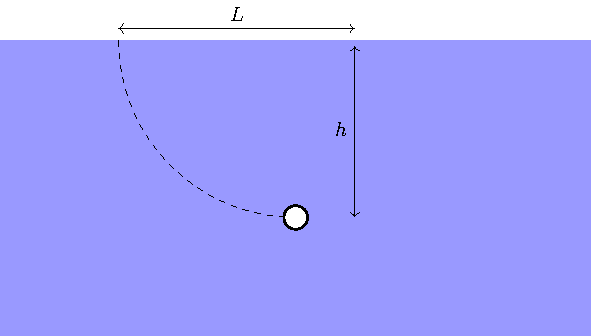
\includegraphics{January2023/1-1.pdf}
\end{center}

}

\sol{

(a) The force on the bathyscaphe is given by
\begin{align}
    \vb*{F} = -M g \vu*{y} - \gamma \vb*{v} + \rho g \Big( \frac{4}{3} \pi R^3 \Big) \vu*{y}
,\end{align}
which in components reads
\begin{align}
    M \ddot{x} &= - \gamma \dot{x} \\
    M \ddot{y} &= - M g - \gamma \dot{y} + \frac{4}{3} \pi R^3 \rho g
.\end{align}
We can solve the equation for $x$ simply:
\begin{align}
    \dot{x} + \frac{\gamma}{M} x = v_0 \Rightarrow \dv{t} \Big( e^{(\gamma/M)t} x \Big) = v_0 e^{(\gamma/M)t} \Rightarrow x(t) = \frac{M v_0}{\gamma} ( 1 - e^{-(\gamma / M)t} )
.\end{align}
We can also solve the equation for $y$ in a similar way:
\begin{gather}
    \dot{y} + \frac{\gamma}{M} y = -\frac{\gamma h}{M} - \Big( 1 - \frac{4 \pi R^3 \rho}{3 M} \Big) g t \nonumber \\
    \dv{t} \Big( e^{(\gamma / M) t} y \Big) = -\frac{\gamma h}{M} e^{(\gamma / M)t} - \Big( 1 - \frac{4 \pi R^3 \rho}{3 M} \Big) g t e^{(\gamma / M)t} \nonumber \\
    y(t) = - h - h ( 1 - e^{-(\gamma / M) t} ) - \Big( 1 - \frac{4 \pi R^3 \rho}{3 M} \Big) g e^{-(\gamma / M)t} \int_{0}^{t} \dd{t'} t' e^{(\gamma / M)t'} \nonumber \\
    y(t) = - h - h ( 1 - e^{-(\gamma / M) t} ) - \Big( \frac{M}{\gamma} \Big)^2 \Big( 1 - \frac{4 \pi R^3 \rho}{3 M} \Big) g e^{-(\gamma / M)t} \int_{0}^{\gamma t / M} \dd{x} x e^{x} \nonumber \\
    y(t) = - h - h ( 1 - e^{-(\gamma / M) t} ) - \Big( \frac{M}{\gamma} \Big)^2 \Big( 1 - \frac{4 \pi R^3 \rho}{3 M} \Big) g \Bigg[ \frac{\gamma}{M} t + ( 1 - e^{-(\gamma / M)t} ) \Bigg]
.\end{gather}
Assuming that the time to reach the top $T \gg \gamma / M$, we have
\begin{gather}
    0 = - h - h \frac{\gamma T}{M} + \Big( \frac{M}{\gamma} \Big)^2 \Big( \frac{4 \pi R^3 \rho}{3 M} - 1 \Big) \frac{2 \gamma T}{M} g \nonumber \\
    \eqbox{ T = h \Bigg[ \frac{2 M g}{\gamma} \Bigg( \frac{4 \pi R^3 \rho}{3 M} - 1 \Bigg) - \frac{\gamma h}{M} \Bigg]^{-1} }
.\end{gather}

(b) Using the result above, the lateral distance the bathyscaphe travels before emerging is
\begin{align}
    \eqbox{ L = v_0 T = h v_0 \Bigg[ \frac{2 M g}{\gamma} \Bigg( \frac{4 \pi R^3 \rho}{3 M} - 1 \Bigg) - \frac{\gamma h}{M} \Bigg]^{-1} }
.\end{align}


}


\prob{1.2}{

A thin-shelled sphere of radius $\rho$ and mass $m$ is constrained to roll without slipping on the lower half of the inner surface of a hollow, stationary cylinder of radius $R$.

Take $\theta$ to be the generalized coordinate and use $I = \frac{2}{3} m \rho^2$ to find the Lagrange equation of motion that describes the motion of the shell.

\begin{center}
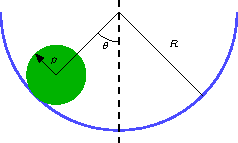
\includegraphics{January2023/1-2.pdf}
\end{center}

}

\sol{

Let us use cylindrical coordinates to write $x = (R - \rho) \sin{\theta}$ and $y = (R - \rho) \cos{\theta}$, where we have oriented $y$ to point down.
The velocity 
\begin{align}
    \vb*{v} = (R - \rho) \dot{\theta} ( \cos{\theta} \vu*{x} - \cos{\theta} \vu*{y} ) + \dot{z} \vu*{z}
.\end{align}
The kinetic energy is then
\begin{align}
    T = \frac{m v^2}{2} + \frac{I \omega^2}{2} = \frac{m v^2}{2} + \frac{1}{2} \frac{2}{5} m \rho^2 \frac{v^2}{\rho^2} = \frac{7 m v^2}{10} = \frac{7 m}{10} \Big[ (R - \rho)^2 \dot{\theta}^2 + \dot{z}^2 \Big]
,\end{align}
so our Lagrangian reads
\begin{align}
    L = \frac{7 m}{10} \Big[ (R - \rho)^2 \dot{\theta}^2 + \dot{z}^2 \Big] + m g (R - \rho) \cos{\theta}
.\end{align}
Notice that $z$ is a cyclic coordinate, so its motion is related to the constant of motion
\begin{align}
    p_{z} = \pdv{L}{\dot{z}} = \frac{7m}{5} \dot{z} \Rightarrow z = z_0 + \frac{5 p_z}{7m} t
.\end{align}
On the other hand, for $\theta$, we have
\begin{align}
    \eqbox{ \ddot{\theta} + \frac{5 g}{7(R - \rho)} \sin{\theta} = 0 }
.\end{align}

}


\prob{1.3}{

An ideal (flexible, uniform, frictionless, etc.) rope of length $l$ and mass $M$ starts sliding off an ideal frictionless table as shown in the figure (the rope is initially at rest, the gravitational accleration is $g$, the size of the piece of the rope initially hanging off the table is $y_0$).

\begin{center}
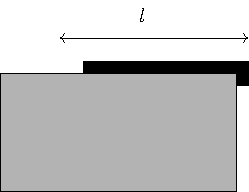
\includegraphics{January2023/1-3.pdf}
\end{center}

\begin{parts}
    \item Introduce some generalized coordinate and write down the Lagrangian of the system.

    \item Derive the Euler-Lagrange equations of motion.

    \item Calculate the time $\tau$ for the rope to slide half-way off the table.
\end{parts}

}

\sol{

(a) Let $y$ denote the length of rope hanging off the table.
The kinetic energy of the rope is then 
\begin{align}
    T = \int \frac{\dd{m} \dot{y}^2}{2} = \frac{M \dot{y}^2}{2}
.\end{align}
The potential energy is just
\begin{align}
    U = -\int \dd{m} g y' = -\rho g \int_0^{y} y' \dd{y'} = -\frac{M g y^2}{2 l}
.\end{align}
Putting these together, our Lagrangian
\begin{align}
    \eqbox{ L = \frac{M \dot{y}^2}{2} + \frac{M g y^2}{2 l} }
.\end{align}

(b) This Lagrangian yields the equation of motion
\begin{align}
    \eqbox{ \ddot{y} - \frac{g}{l} y = 0 }
,\end{align}
which has solution
\begin{align}
    y(t) = y_0 \cosh(\frac{g t}{l})
.\end{align}

(c) The time $\tau$ for the rope to be halfway off the table is defined through
\begin{align}
    y(\tau) = \frac{l}{2} \Rightarrow \eqbox{ \tau = \frac{l}{g} {\rm arcosh}\Big( \frac{y_0}{2 l} \Big) }
.\end{align}

}


\prob{1.4}{

A smooth wire is bent into the shape of a spiral helix with a decreasing pitch.
In cylindrical polar coordinates $(\rho,\phi,z)$ it is specified by equations $\rho = R$ and $z = \lambda \sqrt{\phi}$, where $R$ and $\lambda$ are positive constants.
The $z$ axis is vertically up (and gravity vertically down).

\begin{parts}
    \item Using $z$ as a generalized coordinate, write down the Lagrangian for a bead of mass $m$ threaded on the wire.

    \item Find the Lagrange equation and calculate the bead's vertical acceleration $\ddot{z}$ as a function of $z$ and $\dot{z}$.

    \item Find aceleration $\ddot{z}$ in two limits: (i) when $R \rightarrow 0$ but $\lambda$ is fixed, and (ii) when $\lambda \rightarrow \infty$ but $R$ is fixed.
    Discuss if the results for $\ddot{z}$ in these limits make sense.
\end{parts}

}

\sol{

In cylindrical coordinates
\begin{align}
    \eqbox{ L = \frac{m}{2} \Big[ R^2 \dot{\phi}^2 + \dot{z}^2 \Big] - m g z = \frac{m}{2} \Big( 1 + \frac{4 R^2 z^2}{\lambda^{4}} \Big) \dot{z}^2 - m g z }
.\end{align}

(b) The equation of motion is just
\begin{gather}
    \eqbox{ m \Big( 1 + \frac{4 R^2 z^2}{\lambda^{4}} \Big) \ddot{z} + \frac{8 R^2 z \dot{z}^2}{\lambda^{4}} + mg = 0 }
.\end{gather}


(c) In the limit $R \rightarrow 0$ with fixed $\lambda$, our acceleration is just $\ddot{z} = -g$.
In the second limit $\lambda \rightarrow \infty$ with fixed $R$, we have $\ddot{z} = -g$.

}


\prob{2.1}{

You are told that, at the known positions $x_1$ and $x_2$, an oscillating mass $m$ has speeds $v_1$ and $v_2$.
What are the amplitude and the angular frequency of the oscillations?

}

\sol{

The position as a function of time
\begin{align}
    x(t) = A \cos(\omega t + \gamma)
,\end{align}
and solving for $t$, we find
\begin{align}
    t = \frac{1}{\omega} \Big[ \arccos(\frac{x}{A}) - \gamma \Big]
.\end{align}
Putting this into the expression for velocity, we have
\begin{align}
    |\dot{x}| = A \omega | \sin(\omega t + \gamma) | = A \omega \Big|\sin(\arccos(\frac{x}{A}))\Big| = \omega \sqrt{A^2 - x^2}
.\end{align}
Using the boundary conditions, we have the system of equations
\begin{align}
    v_1 &= \omega \sqrt{A^2 - x_1^2} \\
    v_2 &= \omega \sqrt{A^2 - x_2^2}
.\end{align}
Thus
\begin{align}
    \eqbox{ A = \sqrt{\frac{v_2^2 x_1^2 - v_1^2 x_2^2}{v_2^2 - v_1^2}}, \quad \omega = \sqrt{\frac{x_1^2 - x_2^2}{v_2^2 - v_1^2}} }
.\end{align}

}

\subsection*{Electricity \& Magnetism}
\addcontentsline{toc}{subsection}{Electricity \& Magnetism}

\prob{2.2}{

An electron with mass $m_e$ and momentum $p_e$ hits a positron at rest.
They annihilate, producing a pair of photons.
If one of the photons emerge at angle $\theta$ to the incident electron direction, what is the second photon's angle?

}

\sol{

From the conservation of energy and 3-momentum, we have the set of equations
\begin{align}
\begin{cases}
    E + m_e = E_\gamma + E_{\gamma}' \\
    p_e = E_\gamma \cos{\theta} + E_{\gamma}' \cos{\theta'} \\
    0 = E_\gamma \sin{\theta} - E_{\gamma}' \sin{\theta'}
.\end{cases}
\end{align}
From the last equation, we can write
\begin{align}
    E_{\gamma} = E_{\gamma'} \frac{\sin{\theta'}}{\sin{\theta}}
.\end{align}
Putting this into the second equation,
\begin{align}
    p_{e} = E_{\gamma'} \Big( \cot{\theta} \sin{\theta'} + \cos{\theta'} \Big) \Rightarrow E_{\gamma}' = \frac{p_{e}}{\cot{\theta} \sin{\theta'} + \cos{\theta'}}
.\end{align}
Putting this into the first equation, we find
\begin{gather}
    E + m_{e} = \frac{p_{e}}{\cot{\theta} \sin{\theta'} + \cos{\theta'}} \Big( 1 + \frac{\sin{\theta'}}{\sin{\theta}} \Big) \nonumber \\
    \frac{E + m_{e}}{p_{e}} = \frac{\sin{\theta} + \sin{\theta'}}{\cos{\theta}\sin{\theta'} + \sin{\theta} \cos{\theta'}} 
.\end{gather}
Solving for $\sin{\theta'}$, we find
\begin{align}
    \frac{\sin{\theta'}}{\sin{\theta}} = \frac{(A \cos{\theta} - 1) \pm A ( A - \cos{\theta} )}{1 + A^2 - 2 A \cos{\theta}}
,\end{align}
where $A = (E + m_{e})/p_{e}$.
There are two solutions here, where the $-$ yields that the two photons go off together in the same direction, leaving us with
\begin{align}
    \eqbox{ \frac{\sin{\theta'}}{\sin{\theta}} = \frac{A^2 - 1}{1 + A^2 - 2A \cos{\theta}} = \frac{(E + m_{e})^2 - p_{e}^2}{p_{e}^2 + (E + m_{e})^2 - 2 p_{e} (E + m_{e}) \cos{\theta}} = \frac{m_{e}}{E - p_{e} \cos{\theta}} }
.\end{align}

}


\prob{2.3}{

A toroid is a ``donut'' shaped coil, and the figure below shows an overhead cross sectional view of one.
They are used in nuclear fusion reactors called tokamaks.
Use Ampere's law to derive the equation for the magnitude of the magnetic field in a toroid ($N$ turns) of inner radius $a$ and outer radius $b$ at a distance $r$ midway between $a$ and $b$.

Express your result in terms of $a$, $b$, current $I$, $N$ and any constants.

\begin{center}
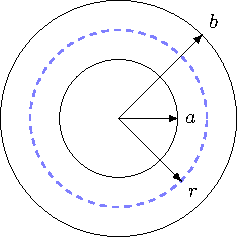
\includegraphics{January2023/2-3.pdf}
\end{center}

}

\sol{

If we take our Amperian loop as shown by the dotted blue line, then
\begin{align}
    B(2 \pi r) = \mu_0 N I \Rightarrow \eqbox{ \vb*{B} = \frac{\mu_0 N I}{2 \pi r} \vu*{\phi} }
.\end{align}

}


\prob{2.4}{

A small neutral metallic conducting sphere with radius $a$ is separated by a transverse distance $R \gg a$ from an infinitely long wire of negligible thicknes and charge per unit length $\lambda$.

\begin{center}
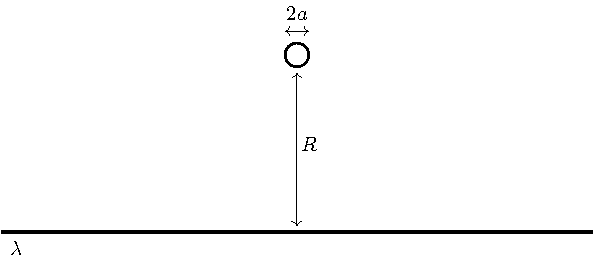
\includegraphics{January2023/2-4.pdf}
\end{center}

Calculate the force between the metallic sphere and the wire.

\textbf{Hint}: Recall the induced electric dipole moment of a conducting sphere in a uniform electric field $\vb*{E}$ is $\vb*{p} = 4 \pi a^3 \vb*{E}$.

}

\sol{

If we assume that $a \ll R$, then we can treat the field produced by the wire as uniform enough to induce a dipole over the sphere.
Such a field is determined by Gauss' law to be
\begin{align}
    \vb*{E} = \frac{\lambda}{2 \pi \epsilon_0 r} \vu*{r}
,\end{align}
where $r$ is the distance from the wire.
The induced dipole is then just
\begin{align}
    \vb*{p} = 4 \pi \epsilon_0 a^3 \vb*{E} = \frac{2 \lambda a^3}{R} \vu*{r}
.\end{align}
The force on sphere by the wire is then just
\begin{align}
    \eqbox{ \vb*{F} = ( \vb*{p} \cdot \grad ) \vb*{E} = \frac{2 \lambda a^3}{R} \pdv{\vb*{E}}{r} = -\frac{2 \lambda a^3}{R} \frac{\lambda}{2 \pi \epsilon_0 R^2} \vu*{r} = -\frac{\lambda^2 a^3}{\pi \epsilon_0 R^3} \vu*{r} }
.\end{align}


}


\prob{3.1}{

The $\psi'$ particle, which is a bound state $\bar{c}c$ of charmed quarks, has mass approximately equal to $3.7~{\rm GeV}/c^2$.

What is the minimal (``threshold'') energy of photons necessary to produce $\psi'$ particles in the reaction $\gamma p \rightarrow p \psi'$ from the Hall D photon source at JLab accelerator?

}

\sol{

The threshold kinetic energy of the photon for $\psi'$ production is defined such that
\begin{gather}
    \sqrt{s} = \sqrt{m_{p}^2 + 2 m_{p} T_{\rm th}} = m_{\psi'} + m_{p} \nonumber \\
    \eqbox{ T_{\rm th} = m_{\psi'} + \frac{m_{\psi'}^2}{2 m_{p}} \approx 11.7~{\rm GeV} }
.\end{gather}

}


\prob{3.2}{

A cylinder of radius $\rho = a$ carries an azimuthal surface current $\vb*{K} = f(z) \hat{\phi}$ where $f(z)$ is an arbitrary function, in cylindrical coordinate $(\rho,\phi,z)$.

Find expressions for $\vb*{B}(0)$, the magnetic field at the origin, and $\vb*{m}$, the magnetic moment of the system, as integrals involving $f(z)$.

}

\sol{

The Biot-Savart law is given generally by
\begin{align}
    \vb*{B}(\vb*{r}) = \frac{\mu_0}{4 \pi} \int \dd[3]{\vb*{r}'} \frac{\vb*{J}(\vb*{r}') \cross (\vb*{r} - \vb*{r}')}{|\vb*{r} - \vb*{r}'|^3}
.\end{align}
Working in cylindrical coordinates and evaluating at the origin, we have
\begin{align}
    \vb*{B}(\vb*{r}) &= \frac{\mu_0 a}{4 \pi} \int_{0}^{2\pi} \dd{\phi'} \int_{-\infty}^{\infty} \dd{z'} \frac{f(z') \vu*{\phi} \cross - ( a \vu*{s} + z \vu*{z} ) }{(a^2 + z'^2)^{3/2}} \nonumber \\
                     &= \frac{\mu_0 a}{4 \pi} \int_{0}^{2\pi} \dd{\phi'} \int_{-\infty}^{\infty} \dd{z'} \frac{f(z')}{(a^2 + z'^2)^{3/2}} (a \vu*{z} - z \vu*{s}) \nonumber \\
                     &= \eqbox{ \frac{\mu_0 a^2}{2} \vu*{z} \int_{-\infty}^{\infty} \dd{z'} \frac{f(z')}{(a^2 + z'^2)^{3/2}} }
.\end{align}

The magnetic moment of the cylinder is given as
\begin{align}
    \eqbox{ \vb*{m} = \frac{1}{2} \int \dd[3]{\vb*{r}} \vb*{r} \cross \vb*{J}(\vb*{r}) = \frac{a}{2} \int_{0}^{2 \pi} \dd{\phi'} \int_{-\infty}^{\infty} \dd{z'} (a \vu*{s} + z' \vu*{z}) \cross f(z') \vu*{\phi} = \frac{a^2}{2} \vu*{z} \int_{-\infty}^{\infty} f(z') \dd{z'} }
.\end{align}

}


\prob{3.3}{

Consider two semi-infinite dielectric media with permittivities $\epsilon_1$ at $x < 0$ and $\epsilon_2$ at $x > 0$.
Let a charge $q$ be in a medium 1 at $x_0 = -L$, where $L$ is a distance between the charge and the planar interface $x = 0$ between the media.
Calculate:

\begin{parts}
    \item The electric potential $\varphi(x,y,z)$ in the entire space.

    \item The force $F$ acting on the charge.
\end{parts}

\begin{center}
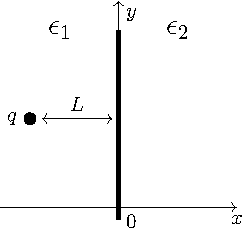
\includegraphics{January2023/3-3.pdf}
\end{center}

}

\sol{

We can construct the potential via the method of images.
For the potential in region 1, let's place an image charge the same distance from the $yz$-plane as the real charge but of magnitude $q'$:
\begin{align}
    \varphi_1 = \frac{1}{4 \pi \epsilon_1} \Bigg[ \frac{q}{\sqrt{(x + L)^2 + \rho^2}} + \frac{q'}{(x - L)^2 + \rho^2} \Bigg]
,\end{align}
where $\rho^2 = y^2 + z^2$.
In the second region, let's replace the charge $q$ with $q''$ to write
\begin{align}
    \varphi_2 = \frac{1}{4 \pi \epsilon_2} \frac{q''}{\sqrt{(x + L)^2 + \rho^2}}
.\end{align}
We can solve for the image charge magnitude $q'$ and $q''$ by enforcing boundary conditions:
\begin{align}
    ( \vb*{D}_{2} - \vb*{D}_{1} ) \cdot \vu*{x} = 0 \Rightarrow q - q' = q'' \\
    ( \vb*{E}_{2} - \vb*{E}_{1} ) \cdot \vu*{\rho} = 0 \Rightarrow \epsilon_2(q + q') = \epsilon_1 q''
.\end{align}
Thus
\begin{align}
    q' = \frac{\epsilon_1 - \epsilon_2}{\epsilon_1 + \epsilon_2} q, \quad q'' = \frac{2 \epsilon_2}{\epsilon_1 + \epsilon_2} q
.\end{align}
From this, we can write
\begin{align}
    \eqbox{ \varphi(x,y,z) = \frac{q}{4 \pi} \begin{cases}
            \displaystyle \frac{1}{\epsilon_1} \Big\{ \frac{1}{\sqrt{(x + L)^2 + y^2 + z^2}} + \frac{\epsilon_1 - \epsilon_2}{\epsilon_1 + \epsilon_2} \frac{1}{\sqrt{(x - L)^2 + y^2 + z^2}} \Big\} & x < 0\\
        \displaystyle \frac{2}{\epsilon_1 + \epsilon_2} \frac{1}{\sqrt{(x + L)^2 + y^2 + z^2}} & x > 0
    \end{cases}
}
.\end{align}

(b) The force on the charge in region 1 is that from the image charge $q'$
\begin{align}
    \vb*{F} = \frac{1}{4 \pi \epsilon_1} \frac{\epsilon_1 - \epsilon_2}{\epsilon_1 + \epsilon_2} \frac{q^2}{(2 L)^2} \vu*{x}
.\end{align}

}

\subsection*{Quantum Mechanics}
\addcontentsline{toc}{subsection}{Quantum Mechanics}

\prob{3.4}{

A particle with spin $S = 1$ is in a state described by the following bra-vector in the $\hat{S}_z$ basis:
\begin{align*}
    \bra{\psi} = \frac{1}{\sqrt{14}} (-i,2,3)
\end{align*}

\begin{parts}
    \item Calculate the probabilities that a measurements of $S_z$ wll give 1, 0, and -1.

    \item Calculate the expectation values of $\expval{S_z}$, $\expval{S_y}$, and $\expval{S_z}$.
\end{parts}

\textbf{Hint}: The spin-1 matrices are
\begin{align*}
    \hat{S}_x = \frac{\hbar}{\sqrt{2}}\begin{pmatrix}
        0 & 1 & 0 \\
        1 & 0 & 1 \\
        0 & 1 & 0
    \end{pmatrix}
    ,\quad
    \hat{S}_y = \frac{\hbar}{\sqrt{2}}\begin{pmatrix}
    0 & -i & 0 \\
    i & 0 & -i \\
    0 & i & 0
    \end{pmatrix}
    , \quad
    \hat{S}_z = \hbar
    \begin{pmatrix}
        1 & 0 & 0 \\
        0 & 0 & 0 \\
        0 & 0 & -1
    \end{pmatrix}
\end{align*}

}

\sol{

(a) The probabilities are simply
\begin{align}
    \eqbox{ P(1) = \frac{1}{14}, \quad P(0) = \frac{2}{7}, \quad P(-1) = \frac{9}{14} }
.\end{align}

(b) The expectation values are as follows:
\begin{align}
\eqbox{
\begin{aligned} 
    \expval{S_x} &= \frac{\hbar}{\sqrt{2}} \frac{1}{14} \begin{pmatrix}
        -i & 2 & 3
    \end{pmatrix}
    \begin{pmatrix}
        0 & 1 & 0 \\
        1 & 0 & 1 \\
        0 & 1 & 0
    \end{pmatrix}
    \begin{pmatrix}
    i \\ 2 \\ 3
    \end{pmatrix}
    = \frac{6 \hbar}{7 \sqrt{2}}
\\
        \expval{S_y} &= \frac{\hbar}{\sqrt{2}} \frac{1}{14} \begin{pmatrix}
        -i & 2 & 3
    \end{pmatrix}
    \begin{pmatrix}
        0 & -i & 0 \\
        i & 0 & -i \\
        0 & i & 0
    \end{pmatrix}
    \begin{pmatrix}
    i \\ 2 \\ 3
    \end{pmatrix}
    = 0
\\
            \expval{S_z} &= \hbar \Big[ \frac{1}{14} - \frac{9}{14} \Big] = -\frac{4 \hbar}{7}
\end{aligned}
}
.\end{align}

}


\prob{4.1}{

Consider a particle of mass $m$ subject to a $\delta$-function potential given by
\begin{align*}
    V(x) = -\frac{\hbar^2}{2m} v_0 \delta(x)
.\end{align*}
Suppose the particle is initially in the bound state.
Suddenly, the potential $V(x)$ is changed to $\overline{V}(x)$ by increasing the strength $v_0 \rightarrow \overline{v}_0$.
Assume that this sudden change does not affect the state of the particle.
Compute the probability that the particle remains in the ground state corresponding to the potential $\overline{V}(x)$.
Why is this probability less than one?

Evaluate the expectation value of the Hamiltonian with the potential $\overline{V}(x)$ and obtain the energy required to change $V(x) \rightarrow \overline{V}(x)$.

}

\sol{

The time-independent Schr\"{o}dinger equation reads
\begin{align}
    -\frac{\hbar^2}{2m} \dv[2]{\psi}{x} - \frac{\hbar^2}{2m} v_0 \delta(x) \psi(x) = E \psi(x)
.\end{align}
If we consider $E < 0$, then the bound state solution takes the form
\begin{align}
    \psi(x) = \begin{cases}
        A e^{\kappa x} & x < 0 \\
        B e^{-\kappa x} & x > 0
    ,\end{cases}
\end{align}
where $\kappa = \sqrt{2 m |E| / \hbar^2}$.
We relate $\kappa$ and $A,B$ by using the following boundary conditions:
\begin{align}
    \psi(0^{-}) = \psi(0^{+}) \Rightarrow A = B \\
    \psi(0^{+}) - \psi(0^{-}) = v_0 \psi(0) \Rightarrow 2 A \kappa = v_0 A \Rightarrow \kappa = \frac{v_0}{2}
.\end{align}
Thus,
\begin{align}
    \psi(x) = \sqrt{\kappa} e^{-\kappa |x|}
.\end{align}
The probability that the after the sudden change, the particle is measured to be in the ground state of the new potential is given by
\begin{align}
    \eqbox{ P = \Bigg| \sqrt{\kappa \bar{\kappa}} \int_{-\infty}^{\infty} \dd{x} e^{-(\kappa + \bar{\kappa}) |x|} \Bigg|^2 = \frac{4 \kappa^2 \bar{\kappa}^2}{(\kappa + \bar{\kappa})^2} = \frac{v_0^2 \bar{v}_0^2}{(v_0 + \bar{v}_0)^2} }
.\end{align}
Note that the probability is less than one because the completeness of states for the second potential includes the continuum of states, whose overlap with the initial state is not necessarily zero.

The expectation value of the Hamiltonian in the new potential is
\begin{align}
    \expval{H} &= -\frac{\hbar^2 \kappa}{2m} \int_{-\infty}^{\infty} \dd{x} e^{-\kappa |x|} \Bigg[ \dv[2]{x} + \bar{v}_0 \delta(x) \Bigg] e^{-\kappa |x|} \nonumber \\
               &= -\frac{\hbar^2 \kappa}{2m} \Bigg[ \kappa^2 \int_{-\infty}^{\infty} \dd{x} e^{- 2 \kappa |x|} + \bar{v}_0 \Bigg] = -\frac{\hbar^2 v_0}{4 m} \Big( \frac{v_0}{2} + \bar{v}_0 \Big) = E - \frac{\hbar^2 v_0 \bar{v}_0}{4m}
.\end{align}
The energy required to change our Hamiltonian as prescribed is then
\begin{align}
    \eqbox{ \Delta E = \frac{\hbar^2 v_0 \bar{v}_0}{4m} = \frac{2 \bar{v}_0}{v_0} |E| }
.\end{align}

}


\prob{4.2}{

Consider a hydrogen atom exposed to a uniform electric field $\mathcal{E} \hat{z}$ (ignore spin degrees of freedom).
Calculate the corrections to the ground-state energy level up to second order in perturbation theory.
You may neglect the contribution from the continuum states in the second-order calculation.

Exploiting selection rules based on parity and $L_z$, you will realize that you only need the following ground- and excited-state wave functions to carry out this calculation,
\begin{align*}
    \phi_{100}(r) = R_{10}(r) \underbrace{\frac{1}{\sqrt{4 \pi}}}_{Y_{00}}, \quad \phi_{n10}(r) = R_{n1}(r) \underbrace{\sqrt{\frac{3}{4 \pi}} \cos{\theta}}_{Y_{10}}
\end{align*}
Express the result in terms of the overlap integral
\begin{align*}
    \gamma_n = \int_{0}^{\infty} \dd{r} \, r^3 R_{n1}(r) R_{10}(r)
.\end{align*}
Note that you do not need to evaluate this integral!

}

\sol{

The first order correction vanishes:
\begin{align}
    E_1^{(1)} = \mel{\phi_{100}}{q \mathcal{E} z}{\phi_{100}} = q \mathcal{E} \mel{\phi_{100}}{z}{\phi_{100}} = 0
,\end{align}
where the expectation value of $z$ vanishes because of parity selection rules.
Thus, we must go to second order to see if we have a nonvanishing correction:
\begin{align}
    E_1^{(2)} = \sum_{nlm \ne 100} \frac{|\mel{\phi_{nlm}}{q E z}{\phi_{100}}|^2}{\epsilon_1 - \epsilon_n} = \frac{q^2 E^2}{\epsilon_1} \sum_{nlm \ne 100} \frac{1}{1 - 1/n^2} |\mel{\phi_{nlm}}{z}{\phi_{100}}|^2
.\end{align}
All that remains is to determine the matrix elements in the sum:
\begin{align}
    \mel{\phi_{nlm}}{z}{\phi_{100}} &= \int \dd[3]{\vb*{r}} R_{nl}(r) Y_{lm}^{*}(\Omega) z R_{10}(r) Y_{10}(\Omega) = \frac{1}{3} \delta_{l 1} \delta_{m 0} \int_{0}^{\infty} \dd{r} r^3 R_{n_1}(r) R_{10}(r) \nonumber \\
    &= \frac{\gamma_n}{3} \delta_{l1} \delta_{m 0}
.\end{align}
Thus
\begin{align}
    \eqbox{ E_1^{(2)} = \frac{q^2 E^2}{3 \epsilon_1} \sum_{n=2}^{\infty} \frac{\gamma_n^2}{1 - 1/n^2} }
.\end{align}

}


\prob{4.3}{

Consider a system with a three-dimensional state space.
The Hamiltonian $\hat{H}$ has a non-degenerate eigenvalue $E_1$ with (normalized) eigenstate $\ket{\phi_1}$ and a degenerate eigenvalue $E_2$ with (orthonormal) eigenstates $\ket{\phi_2}$ and $\ket{\phi_3}$.
Suppose at time $t = 0$, the system is in the normalized state $\ket{\psi(0)}$ given by
\begin{align*}
    \ket{\psi(0)} = \frac{1}{\sqrt{2}} \ket{\phi_1} + \frac{1}{2} ( \ket{\phi_2} + \ket{\phi_3} )
.\end{align*}

\begin{parts}
    \item At $t = 0$ the energy of the system is measured.
    What values can be found and with what probabilities?

    \item Suppose at $t = 0$, instead of $\hat{H}$, the observable $\hat{A}$, which in the basis $\ket{\phi_1}$, $\ket{\phi_2}$, and $\ket{\phi_3}$ is represented by the following matrix
    \begin{align*}
        A = a \begin{pmatrix}
            1 & 0 & 0 \\
            0 & 0 & 1 \\
            0 & 1 & 0
        \end{pmatrix}
    ,\end{align*}
    where $a > 0$ is real, is measured with the system in state $\ket{\psi(0)}$.
    What results can be found and with what probabilities?
    Do $\hat{H}$ and $\hat{A}$ commute?

    \item What is the mean value $\bra{\psi(t)} \hat{A} \ket{\psi(t)}$?
\end{parts}

}

\sol{

(a) We have
\begin{align}
    P(E_1) = \frac{1}{2}, \quad P(E_2) = \frac{1}{2}
.\end{align}

(b) Notice that the state $\ket{\phi_1}$ is already an eigenstate of $A$ with eigenvalue $a$, so we only have to diagonalize the block representing the subspace $\{ \ket{\phi_2}, \ket{\phi_3} \} $:
\begin{align}
    \begin{vmatrix}
        -\lambda & 1 \\
        1 & -\lambda
    \end{vmatrix}
    = \lambda^2 - 1 = 0 \Rightarrow \lambda = \pm 1
.\end{align}
The corresponding eigenvectors and eigenvalues of $A$ are then
\begin{align}
    \pm a \Leftrightarrow \ket{\chi_{\pm}} = \frac{1}{\sqrt{2}} ( \ket{\phi_2} \pm \ket{\phi_3} )
.\end{align}
Using these states, we can write
\begin{align}
    \ket{\psi(0)} = \frac{1}{\sqrt{2}} \ket{\phi_1} + \frac{1}{\sqrt{2}} \ket{\chi_+}
.\end{align}
From this we can see that, a measurement of the system can yield
\begin{align}
    P(a) = 1, \quad P(-a) = 0
.\end{align}

(c) First, we write
\begin{align}
    \ket{\psi(t)} = \frac{1}{\sqrt{2}} e^{-i E_1 t / \hbar} \ket{\phi_1} + \frac{1}{2} e^{-i E_2 t / \hbar} ( \ket{\phi_2} + \ket{\phi_3} )
.\end{align}
Thus, the expectation value
\begin{align}
    \expval{A}{\psi(t)} = a
,\end{align}
which is time independent since $\ket{\psi(t)}$ is an eigenstate of $A$ with eigenvalue $a$ at all times $t$.

}


\prob{4.4}{

Consider a system with a two-dimensional state space.
In this space, the states $\ket{1}$ and $\ket{2}$ form an orthonormal basis.
The Hamiltonian describing the system in this basis has the form
\begin{align*}
    \hat{H} = H_{11} \ket{1}\bra{1} + H_{22} \ket{2}\bra{2} + H_{12} ( \ket{1}\bra{2} + \ket{2}\bra{1} )
,\end{align*}
where $H_{11}$, $H_{22}$, and $H_{12}$ are real parameters with dimension of energy.

\begin{parts}
    \item Assume $H_{12} = 0$.
    Write down the eigenvalues and eigenvectors of $\hat{H}$ in the basis $\ket{1}$, $\ket{2}$.

    \item Now, assume $H_{12} \ne 0$.
    Obtain the eigenvalues and corresponding eigenvectors of $\hat{H}$.
    Make sure that they reduce to the eigenvalues and eigenvectors of part (a) above in the limit $H_{12} \rightarrow 0$.
    It is convenient to introduce the parameter
    \begin{align*}
        \lambda = \frac{2 H_{12}}{H_{11} - H_{22}} \quad {\rm with}~ H_{11} \ne H_{22}
    ,\end{align*}
    and express results in terms of $\lambda$.
\end{parts}

}

\sol{

(a) The Hamiltonian as a matrix in the basis $\{ \ket{1}, \ket{2} \}$
\begin{align}
    H = \begin{pmatrix}
        H_{11} & H_{12} \\
        H_{12} & H_{22}
    \end{pmatrix}
.\end{align}
If $H_{12} = 0$, then the matrix is already diagonal with spectrum
\begin{align}
    \eqbox{ H_{11} \leftrightarrow \ket{1}, \quad H_{22} \leftrightarrow \ket{2} }
.\end{align}


(c) Assuming that the off-diagonal elements are nonzero, we diagonalize via the standard procedure:
\begin{align}
\eqbox{
\begin{aligned}
    E_{\pm} &= \frac{(H_{11} + H_{22}) \pm \sqrt{(H_{11} - H_{22})^2 + 4 H_{12}^2}}{2} \nonumber \\
    &= \frac{1}{2} \Bigg[ ( H_{11} + H_{22} ) \pm |H_{11} - H_{22}| \Big( 1 + \frac{\lambda^2}{2} + \hdots \Big) \Bigg]
,\end{aligned}
}
\end{align}
where $\lambda$ is as prescribed above.
Note that the last equality arises from the limit that the off-diagonal elements are much smaller than the difference of the diagonal ones.
This result reduces to that of part (a) if $\lambda = 0$.

}
